\documentclass[25pt, a0paper, portrait]{tikzposter}
\usepackage[utf8]{inputenc}
\usepackage{authblk}
\usepackage{amsmath}

\usepackage[backend=biber,style=authoryear,sorting=ynt]{biblatex}
\AtEveryBibitem{%
  \clearfield{issn} % Remove issn
  \clearfield{doi} % Remove doi
  \clearfield{title} % Remove title

  \ifentrytype{online}{}{% Remove url except for @online
    \clearfield{url}
  }
}
\addbibresource{document.bib}

\makeatletter
\renewcommand\maketitle{\AB@maketitle} % revert \maketitle to its old definition
%\renewcommand\AB@affilsepx{\quad\protect\Affilfont} % put affiliations into one line
\makeatother
\renewcommand\Affilfont{\small} % set font for affiliations

\title{\parbox{\linewidth}{\huge\centering Temperature effect on neutron capture in tin isotopes}}

\author[1]{\Large A. C. Berceanu}
\author[1, 2]{\Large Y. F. Niu}
\author[1]{\Large Y. Xu}

\affil[1]{ELI-NP, “Horia Hulubei” National Institute for Physics and Nuclear Engineering,
30 Reactorului Street, RO-077125, Bucharest-Magurele, Romania}
\affil[2]{School of Nuclear Science and Technology, Lanzhou University, Lanzhou 730000, China}

% todo: remove
\usepackage{blindtext}
%\usepackage{comment}

\usetheme{Board}


\begin{document}

\maketitle
\node[anchor=west] at (TP@title.west) {
\includegraphics[width=10cm]{images/eli_logo.pdf}};
\node[anchor=east] at (TP@title.east) {
\includegraphics[width=10cm]{images/ifin_logo.pdf}};
%\node[anchor=west,yshift=-2cm] at (TP@title.west) {
\includegraphics[width=10cm]{images/eli_logo.pdf}};
%\node[anchor=east,yshift=-1cm] at (TP@title.east) {
\includegraphics[width=10cm]{images/eli_logo.pdf}};


%\note[targetoffsetx=-9cm, targetoffsety=-6.5cm, width=0.5\linewidth]{e-mail \texttt{welcome@overleaf.com}}

\begin{columns}
    \column{0.5}

    \block{r-process}
    {The r-process nucleosynthesis is responsible for the creation of about half of
    the atomic nuclei heavier than iron, under extreme density and temperature
    conditions. As such, the temperature dependence of neutron capture cross
    sections and rates is important for determining the reaction dynamics. As shown
    by the sensitivity study in~\cite{Mumpower2016}, neutron capture dynamics
    on Sn isotopes are very important for r-process study.  So in this work, we
    study the effect of finite temperature on the neutron-capture cross sections and
    rates of even-even tin isotopes, with neutron numbers between 76 and 96.
	\begin{tikzfigure}
	    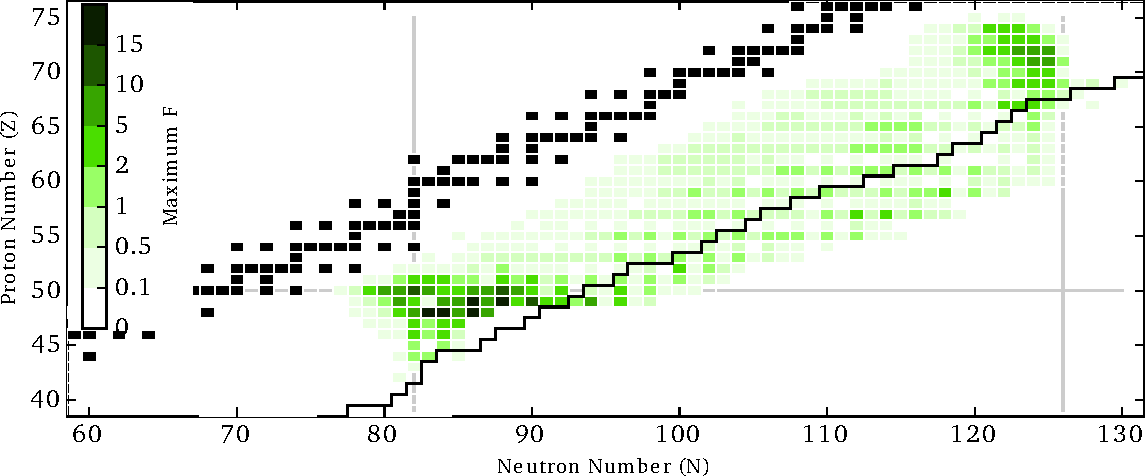
\includegraphics[width=0.4\textwidth]{images/mumpower.pdf}
	\end{tikzfigure}
   }

	\block{Relativistic RPA at finite temperature}{

We compute the E1 dipole strengths, for both zero and finite temperature, using
    relativistic Hartree-Bogoliubov (RHB) + quasiparticle random phase approximation
    (QRPA) and finite-temperature relativistic mean-field (FTRMF) +
    finite-temperature random-phase approximation (FTRPA), respectively.  The same relativistic density functional is used for the mean field in FTRMF and for the residual two-body interaction in FTRRPA. The density-dependent meson-nucleon couplings are used in the relativistic Lagrangian, and we use the parameter set DD-ME2 \cite{Lala, Niu2009}.

	\begin{equation*}
	   \left( \begin{array}{cc} A & B \\ -B^* & -A^* \end{array} \right)
	   \left( \begin{array}{c} X \\ Y \end{array} \right)
	   = \hbar\omega \left( \begin{array}{c} X \\ Y \end{array} \right) \;,
	\end{equation*}
	where
	\begin{equation*}
	   A = \left( \begin{array}{cc} (\epsilon_m - \epsilon_i)
	   \delta_{ii'} \delta_{mm'} &  \\
	   & (\epsilon_\alpha - \epsilon_i) \delta_{\alpha \alpha'}
	   \delta_{ii'} \end{array} \right)
	   + \left( \begin{array}{cc} (n_{i'} - n_{m'})V_{mi'im'} & n_{i'} V_{mi'i\alpha'} \\
	   (n_{i'} - n_{m'})V_{\alpha i' i m'}  &n_{i'} V_{\alpha i' i \alpha'} \end{array}
	   \right) \;,
	  \end{equation*}
	  and
	\begin{equation*}
	   B =\left( \begin{array}{cc} (n_{i'} - n_{m'})V_{mm'ii'} & n_{i'}V_{m\alpha'ii'} \\
	    (n_{i'} - n_{m'})V_{\alpha m' i i'}  & n_{i'}  V_{\alpha \alpha' i i' } \end{array}
	    \right)\; .
	  \end{equation*}

	$V$ is the residual two-body interaction, derived from the relativistic Lagrangian with  density-dependent meson-nucleon couplings \cite{Niksic}. The thermal occupation factors $n_k$ denote a Fermi-Dirac distribution for states in Fermi sea with index $m,i$, and $0$ for states in Dirac sea with index $\alpha$. The configuration space includes not only particle-hole (ph) pairs, but also particle-particle (pp) and hole-hole (hh) pairs. The transition strength for a multipole operator $Q_J$ is

	\begin{equation*}
	   B(J,E_\nu) = \left | \sum_{mi} (X^{\nu,J}_{mi} +
	   (-1)^J Y^{\nu,J}_{mi} ) \langle m || Q_J || i\rangle (n_i
	   -n_m) \right |^2.
	\end{equation*}

	The discrete spectra are averaged with a Lorentzian distribution of an width $\Gamma = 1 $ MeV.
	We use the
    TALYS code for computing the corresponding cross sections, replacing its default
    E1 dipole data.
}

	\block{E1 strength functions}
    {
        \begin{tikzfigure}
            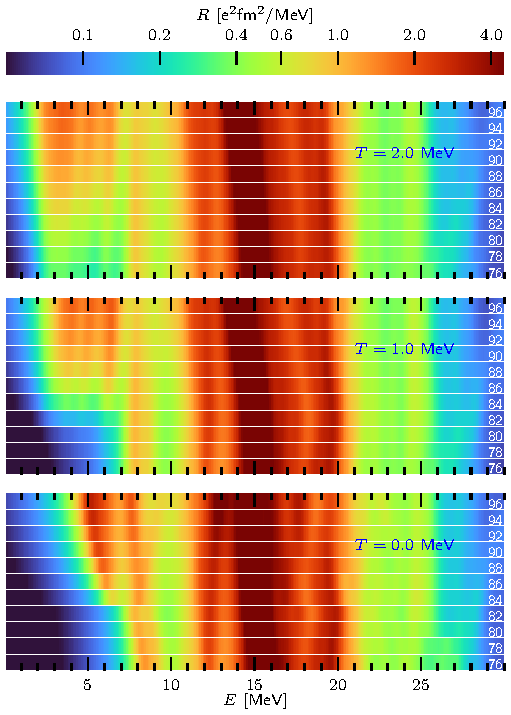
\includegraphics[width=0.4\textwidth]{images/colormesh.pdf}
        \end{tikzfigure}
    }

    \block{References}{
        \printbibliography[heading=none]}


    \column{0.5}

    \block{Cross section}{
        \begin{tikzfigure}
            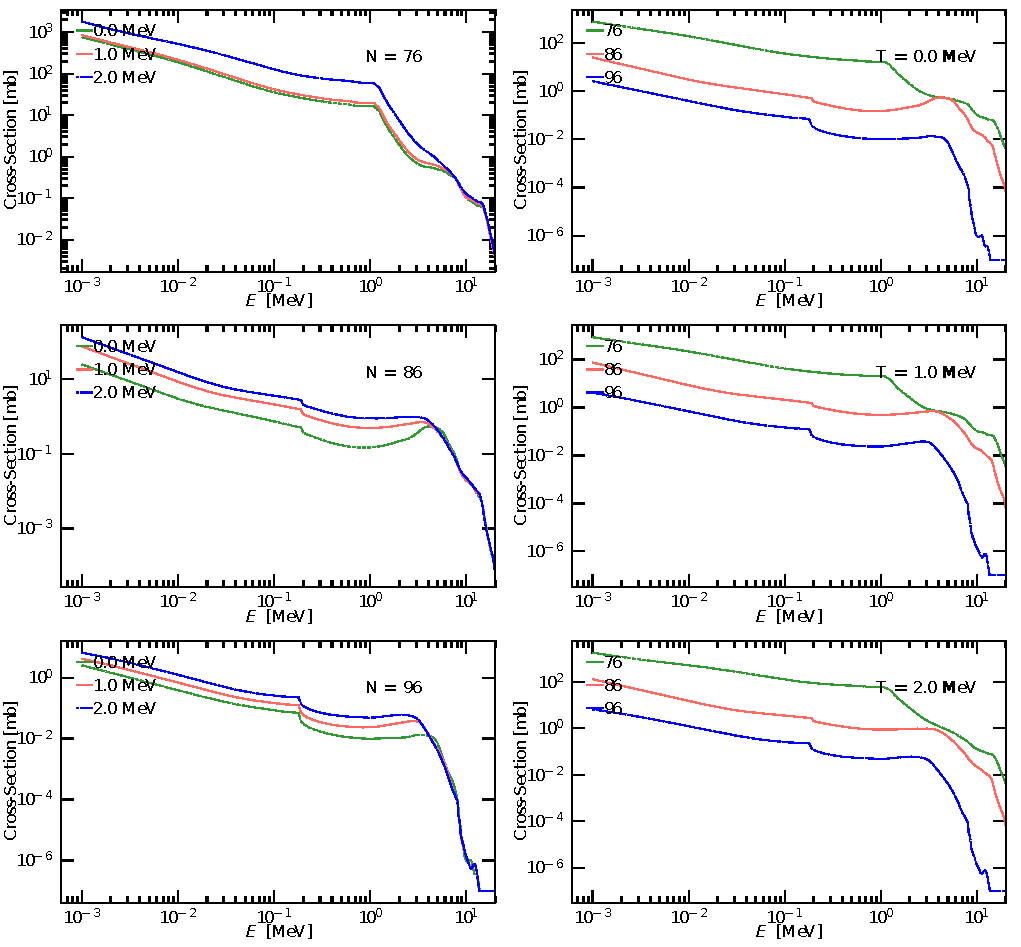
\includegraphics[width=0.4\textwidth]{images/cross_section.pdf}
        \end{tikzfigure}
    }

    \block{Neutron capture rate}{
        \begin{tikzfigure}
            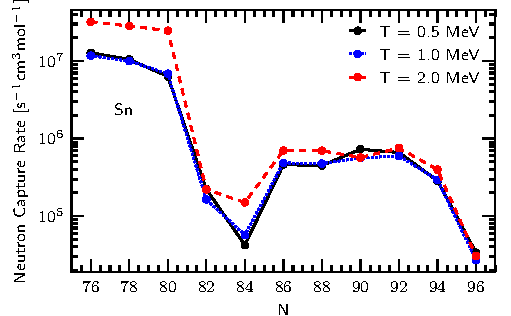
\includegraphics[width=0.4\textwidth]{images/capture_rate_vs_N.pdf}
        \end{tikzfigure}
    }

	\block{E1 strength functions}
    {
        \begin{tikzfigure}
            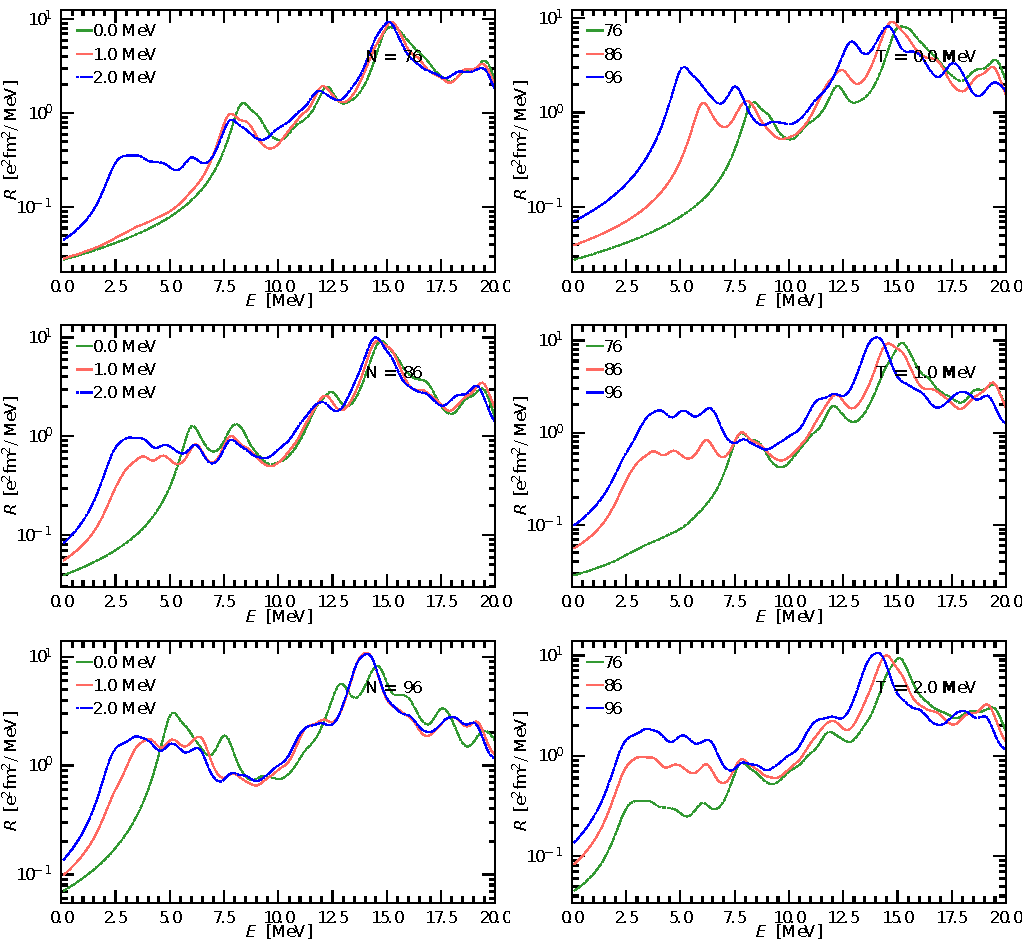
\includegraphics[width=0.4\textwidth]{images/photon_strength_function.pdf}
        \end{tikzfigure}
    }

    \block{~}{
	    Supported by ELI-NP Phase II, a project cofinanced by the 
	    Romanian Government and the EU through the European Regional Development
	    Fund and COP 1/07.07.2016, ID 1334
        \begin{tikzfigure}
            
\includegraphics[width=0.2\textwidth]{images/three_logos.pdf}
        \end{tikzfigure}
	}
\end{columns}

\end{document}
